\subsection{Upload music flowchart}%uploadmusic_flowchart

\begin{figure}[h!]
\centering
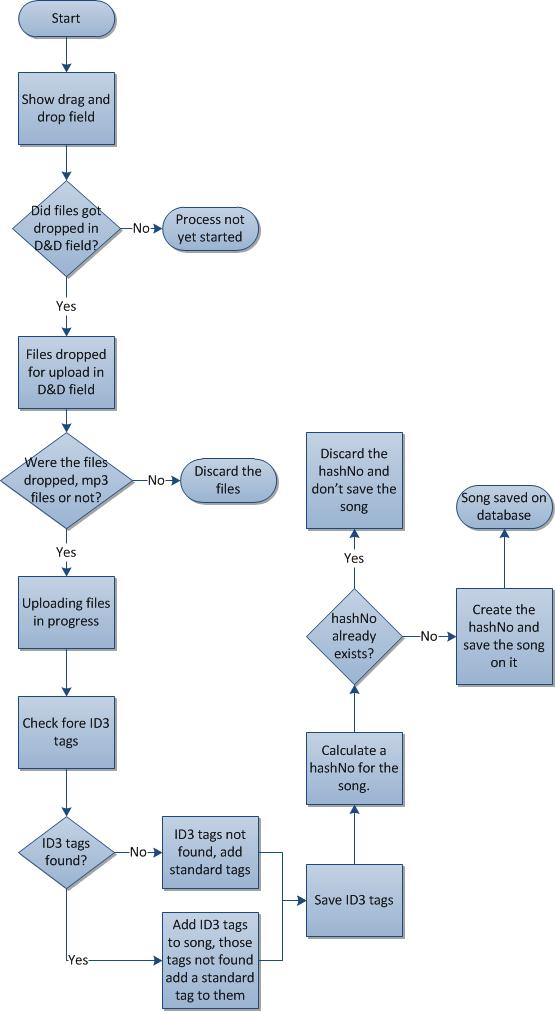
\includegraphics[scale=0.5]{design/figures/uploadmusic_flowchart}
\caption{Flowchart of uploading music to Movingwhales}
\end{figure}%insert picture/figure here

The upload music process consists of the various processes that can be seen in the flowchart diagram. If we go through the steps we can see what happens.
\begin{description}
\item{Step 1:} We are on the upload main site, we can see the field where we have to drag and drop the files to get uploaded. The field has a description on how to upload files.
\item{Step 2:} Behind the scenes the system monitors if there are any files that have been dropped for upload yet. If not nothing happens, if it registers that some files have been dropped for upload we get to.
\item{Step 3:} Where the system has registered that some files have been dropped for upload so it starts to upload the files.
\item{Step 4:} Before the system starts uploading the files it first checks the files if they are of a valid format. If they are not then the files get discarded, else we continue to the next step.
\item{Step 5:} Where the system starts the actual uploading of the files.
\item{Step 6:} While the system is uploading the files, it is checking the files fore ID3 tags at the same time. Then it can go two different ways either.
\item{Step 7a:} If it does not finds ID3 tags, add standard defined tags or
\item{Step 7b:} If it find some ID3 tags, add those tags that were found and give a standard defined tag to those tags not found(e.g. it finds a artist and song name but not an album name).
\item{Step 8:} After the tags have been found they get saved to the song.
\item{Step 9:} Then the process starts to calculate a unique hash number for the uploaded song so it can distinct between the songs. Then it proceed to.
\item{Step 10:} Where it checks for the hash number if it already exists, if it does it goes to
\item{Step 11a:} and merges the sang with the existing one. If it does not exist it goes to
\item{Step 11b:} where it creates the hash number and saves the song to the number. Then it proceeds to saving the song to the database what happens in the last step \textbf{Step 12}.
\end{description}